%FOR PDFLATEX USE ONLY
\documentclass[a4paper,12pt]{article}

\usepackage{amssymb,amsmath} %math symbols

\usepackage[margin=2cm]{geometry} %paper geometry

\usepackage[utf8]{inputenc} %allows unicode (including russian) source file
\usepackage[russian]{babel} %docment in russian-style
\usepackage[utf8]{inputenc}
%\usepackage[unicode]{hyperref} %links inside of the text
\usepackage[pdftex]{graphicx} %includegraphics pictures
\usepackage{cmlgc} %bold text

\usepackage{array} %arrays

%\usepackage{wrapfig}
%\usepackage{array}
%\usepackage{lipsum}
%\usepackage{esvect}
%\usepackage{hyperref}

\usepackage{subfig}
%\usepackage{calc}
%\usepackage{pgfplots,tikz,circuitikz}
%\usepackage{tkz-euclide}

\begin{document}

\begin{center}
  \LARGE{Работа 3.5.3 or 3.2.8}\\[0.2cm]
  \LARGE{Релаксационные колебания}\\[0.2cm]
  \large{Стрижак Даниил}\\[0.2cm]
\end{center}  
  

\section{Аннотация}

В работе предлагается снять вольт-амперную характеристику стабилитрона и познакомиться с работой релаксационного генератора: определить критическое сопротивление, исследовать зависимость периода колебаний от сопротивления при фиксированной ёмкости и от ёмкости при фиксированном сопротивлении.

\section{Теоретические сведения}

 Колебательные системы, как правило, имеют два накопителя, между которыми происходит перекачка энергии. В контуре, содержащем конденсатор и катушку индуктивности, электрическая энергия переходит в магнитную и обратно; при колебаниях маятника потенциальная энергия поля тяжести переходит в кинетическую энергию движущейся массы и т.д. 

\begin{wrapfigure}{r}{0.3\textwidth} 
\begin{center}
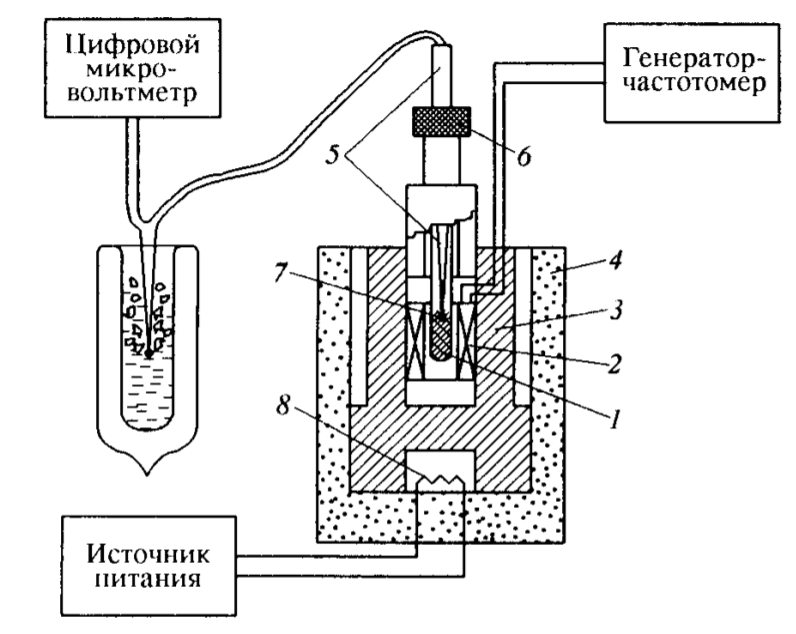
\includegraphics[width=0.3\textwidth]{1.PNG} 
\end{center}
\end{wrapfigure}

Встречаются, однако, колебательные системы, содержащие всего один накопитель энергии. Рассмотрим в качестве примера электрическую цепь, содержащую конденсатор и сопротивление без самоиндукции. Разряд конденсатора через сопротивление представляет собой апериодический процесс. Разряду, однако, можно придать периодический характер, возобновляя заряд конденсатора через постоянные промежутки времени. Колебания в этом случае являются совокупностью двух апериодических процессов - процесса зарядки конденсатора и процесса его разрядки. Такие колебания называются релаксационними.\\
В нашей установке роль ключа, обеспечивающего последовательно попеременную зарядку и разрядку конденсатора, играет газоразрядный диод. Зависимость тока от напряжения для газоразрядной лампы не подчиняется закону Ома и характеризуется рядом особенностей (рис. 1). При малых напряжениях лампа не пропускает тока вовсе (не горит). Ток в лампе возникает только в том случае, если разность потенциалов на её электродах достигает напряжения зажигания $V_{1} .$ При этом, тлеюиций разряд. При дальнейшем незначительном увеличении напряжения сила тока заметно возрастает по закону, близкому к линейному. 
Если начать уменьшать напряжение на горящей лампе, то при напряжении, равном $V_{1},$ лампа ещё не гаснет, и сила тока продолжает уменьшаться. Лампа перестанет пропускать ток лишь при напряжении гашения $V_{2},$ которое обычно существенно меньше $V_{1}$. Сила тока при этом скачком падает от значения $I_{2}\left(I_{2}<I_{1}\right)$ до нуля. Характеристика, изображённая на рис. 1, несколько идеализирована. $\mathrm{Y}$ реальной лампы зависимость $I(V)$ не вполне линейна. При $V>V_{1}$ графики
соответствующие возрастанию и убыванию напряжения, не всегда совпадают. Эти отличия, впрочем, носят второстепенный характер и для нашей задачи несущественны.
 
\newpage

\begin{wrapfigure}{r}{0.3\textwidth} 
\begin{center}
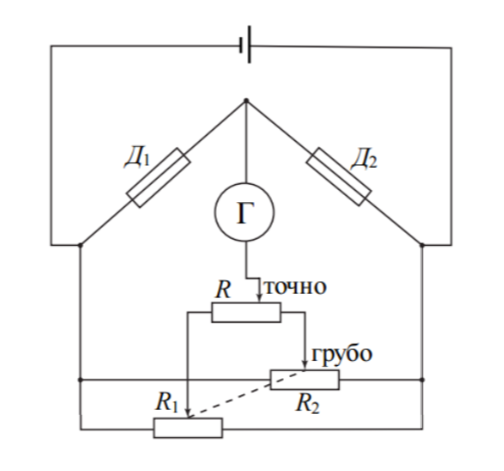
\includegraphics[width=0.3\textwidth]{2.PNG} 
\end{center}
\end{wrapfigure}

\\

Рассмотрим схему релаксационного генератора, представленную на рис. $2 .$ Пусть напряжение бата- реи $U$ больше напряжения зажигания $V_{1} .$ В обозначениях, принятых на схеме, справедливо уравнение

$$I_{C}+I(V)=\frac{U-V}{R}$$

$$C \frac{d V}{d T}+I(V)=\frac{U-V}{R}$$
\\

В стационарном режиме работы, когда напряжение $V$ на конденсаторе постоянно и $d V / d t=0,$ ток через лампу равен

$$I_{\mathrm{cr}}=\frac{U-V}{R}$$

\begin{wrapfigure}{r}{0.3\textwidth} 
\begin{center}
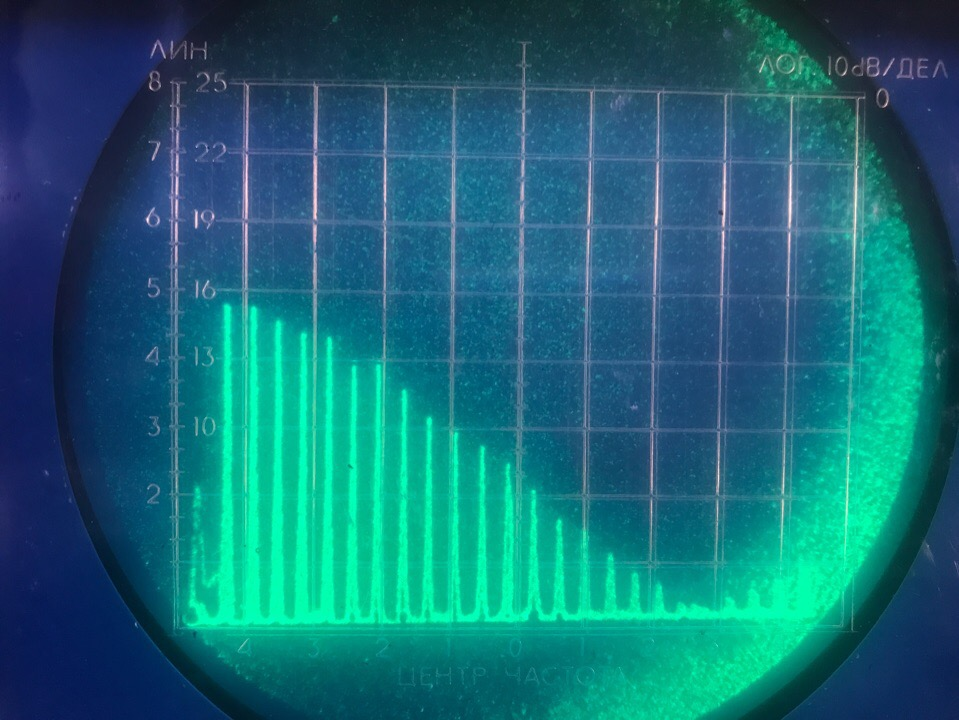
\includegraphics[width=0.3\textwidth]{3.PNG} 
\end{center}
\end{wrapfigure}

Равенство (2) может быть представлено графически (рис. 3) При разных $R$ графрики имеют вид прямых, пересекаЮщихся в точке $V=U, I=0 .$ Область, где эти иагрузочиъе прямвие пересекают вольт-амперную характеристику лампы, соответствует стационарному режиму - при малых $R$ (прямая 1$)$ лампа горит постоянно, колебания Отсутствуют. Прямая $2,$ проходящая через точку $\left(I_{2}, V_{2}\right),$ соответствует критическому сопротивлению
$$
R_{\mathrm{Kp}}=\frac{U-V_{2}}{I_{2}}
$$
При сопротивлении $R>R_{\text {кр }}$ нагрузочная прямая $3 \quad$ не пересекает характеристику лампы, поэтому стационарный режим невозможен. В этом случае в системе устанавливаются колебания. Рассмотрим, как происходит колебательный процесс. Пусть в начале опыта ключ К разомкнут (рис. 2) и $V=0 .$ Замкнём ключ. Конденсатор $C$ начинает заряжаться через сопротивление $R,$ напряжение на нём увеличивается (рис. 4) Как только оно достигнет напряжения зажигания $V_{1},$ лампа начинает проводить ток, причём прохождение тока сопровождается разрядкой конденсатора. В самом деле, батарея $U,$ подключённая через большое сопротивление $R,$ не может поддерживать необходимую для горения лампы величину тока. Во время горения лампы конденсатор разряжается, и когда напряжение на нём достигнет потенциала гашения, лампа перестанет проводить ток, а конденсатор вновь начнёт заряжаться. Возникают релаксационные колебания с амплитудой, равной $\left(V_{1}-V_{2}\right) .$

\newpage

\begin{wrapfigure}{r}{0.3\textwidth} 
\begin{center}
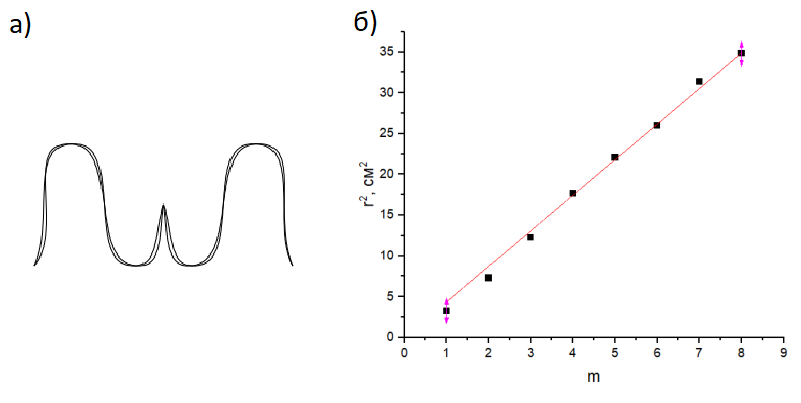
\includegraphics[width=0.3\textwidth]{4.PNG} 
\end{center}
\end{wrapfigure}

Рассчитаем период колебаний. Полное время одного периода колебаний Т состоит из суммы времени зарядки $\tau_{3}$ и времени разрядки $\tau_{\mathrm{p}},$ но если сопротивление $R$ существенно превосходит сопротивление Зажжённой лампы, то $\tau_{3} \gg \tau_{\mathrm{p}}$ и $T \simeq \tau_{3}($ этим случаем мы и ограничимся). Во время зарядки конденсатора лампа не горит $[I(V)=0],$ и уравнение (1) приобретает вид
$$
R C \frac{d V}{d t}=U-V
$$
Будем отсчитывать время с момента гашения лампы, так что $V=V_{2}$ при $t=0$ (рис. 4$) .$ Решив уравнение $(4),$ найдём
$$
V=U-\left(U-V_{2}\right) e^{-t /(R C)}
$$
$\mathrm{B}$ момент зажигания $t=\tau_{3}, V=V_{1},$ поэтому
$$
V_{1}=U-\left(U-V_{2}\right) e^{-\tau_{3} /(R C)}
$$
Из уравнений (5) и (6) нетрудно найти период колебаний:
$$
T \approx \tau_{3}=R C \ln \frac{U-V_{2}}{U-V_{1}}
$$
Развитая выше теория является приближённой. Ряд принятых при расчётах упрощающих предположений оговорен в тексте. Следует иметь в виду, что мы полностью пренебрегли паразитными емкостями и индуктивностями схемы. Не
рассматривались также процессы развития разряда и деионизация при гашении. Поэтому теория справедлива лишь в тех случаях, когда в схеме установлена достаточно большая ёмкость и когда период колебаний существенно больше времени развития разряда и времени деионизации (практически $\gg 10^{-5}$ с). Кроме того, потенциал гашения $V_{2},$ взятый из статической вольт-амперной характеристики, может отличаться от потенциала гашения лампы, работающей в динамическом режиме релаксационных колебаний.

\section{Результаты измерений и обработка данных}
\subsection*{ I. Характеристика стабилитрона}

\begin{wrapfigure}{r}{0.3\textwidth} 
\begin{center}
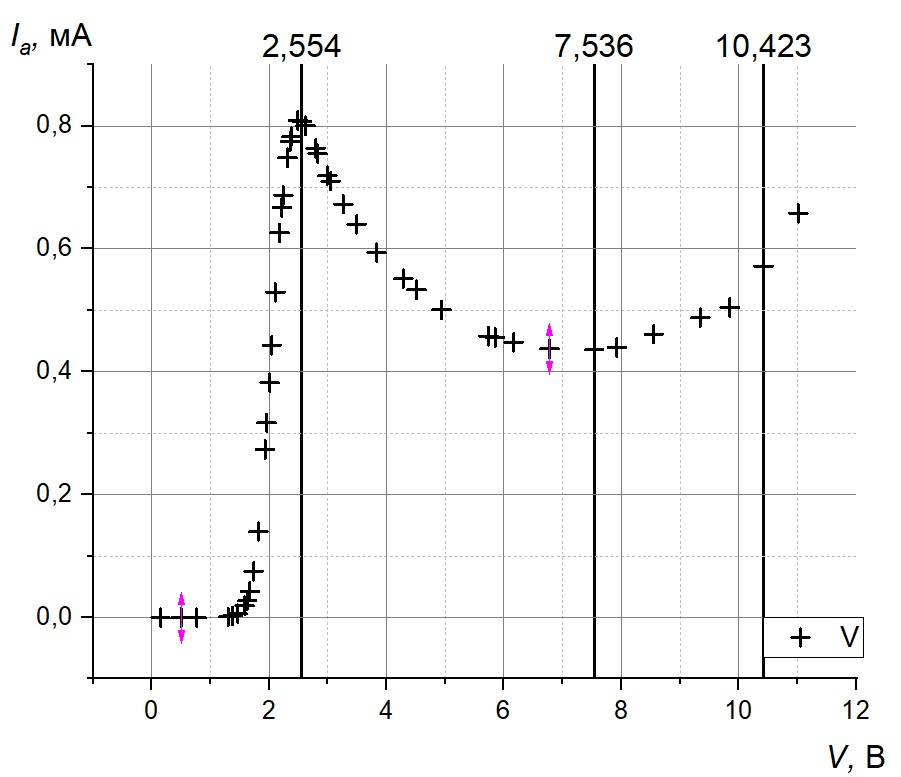
\includegraphics[width=0.3\textwidth]{5.PNG} 
\end{center}
\end{wrapfigure}

Соберем схему, изображённую на рис. 5. Добавочное сопротивление $r$ подпаяно между ножкой лампы и соответствующей клеммой для того, чтобы предохранить стабилитрон от перегорания. Это сопротивление остаётся включённым при всех измерениях. $$r = 5,4\ кOм$$. 
Установим регулятор источника питания на минимум напряжения и включим источник в сеть.\\
Сниием вольтамперную характеристику стабилитрона с резистором $r$ при возрастании и убывании напряжения. При этом как можно точнее определим потенциалы зажигания и гашения $V_{1} = 88,73 В$ и $V_{2} = 80,55 В$ и соответствующие токи $I_{1} = 3,144 А$ и $I_{2} = 1,254 А$

\subsection*{II. Осциллограммы релаксационных колебаний}   
        


\begin{center}
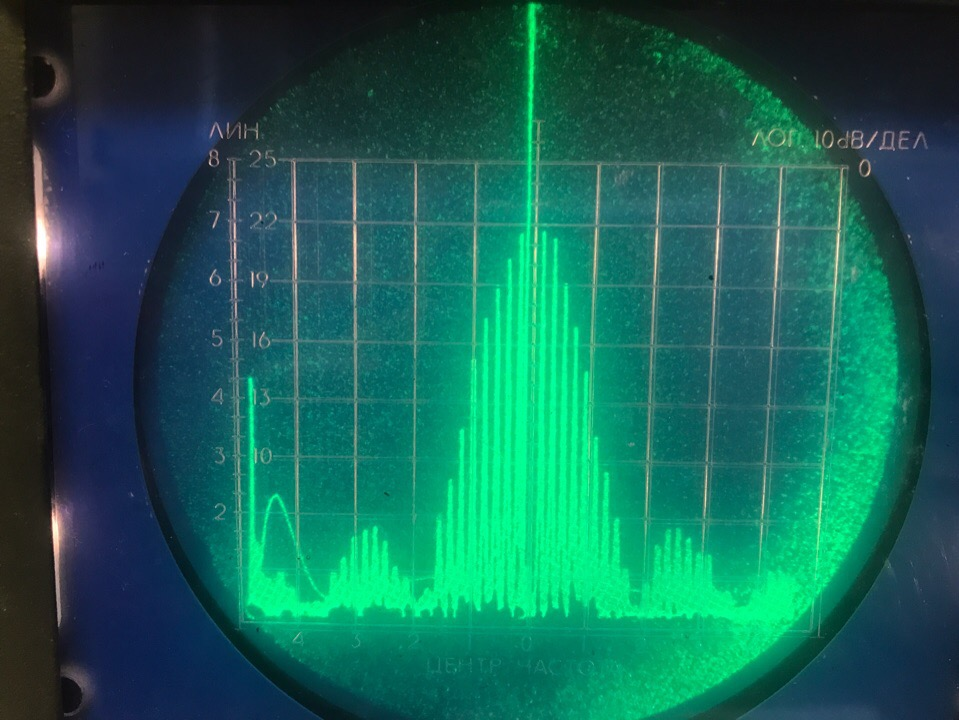
\includegraphics[width=\textwidth]{6.PNG} 
\end{center}


Соберем релаксационный генератор согласно рис. $6 .$
Установим на магазине емкостей значение $C=0,05$ мкФ, а на магазине сопротивлений $R=900$ кОм.\\
Включите в сеть звуковой генератор и источник питания; установите напряжение $U \simeq 1,2 V_{1} = 107 В$ (целое значение, близкое к рассчитанному).\\
Подберём частоту развёртки ЭO, при которой на экране видна картина пилообразных колебаний (рис. 4$)$\\
Получив пилу на экране, оценим соотношение между временем зарядки $\tau_{3}$ и временем разрядки $\tau_{\mathrm{p}} $ , оно равно $\frac{25}2$. При этом картина колебаний выглядит так:\\

\begin{center}
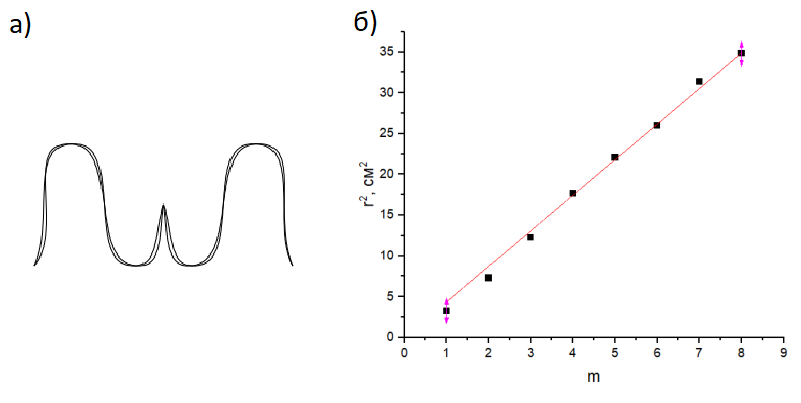
\includegraphics[width=0.3\textwidth]{4.PNG} \\
тут должна быть картинка с осциллографа, но она точно такая же\\
\end{center}

Уменьшая сопротивление магазина, определим $R_{\text {кр }},$ при котором пропадают колебания, и сравните его с величиной, рассчитанной по формуле (3). Это сравнение полезно сделать в процессе работы и подумать о причинах расхождения результатов.\\

$$R_{\text {кр }}  = 78 кОм$$

Колебания пропадают не только при уменьшении $R$ при постоянном $U,$ но и при увеличении $U$ при постоянном $R,$ когда это $R$ не слишком превышает $R_{\mathrm{Kp}}$. \\

При значении $R = 150 кОм$ проведем серию измерений $T = T(C)$ при постоянном напряжении. \\

\begin{minipage}{0.25\textwidth}
\begin{center}
\begin{tabular}{|c|c|}
\hline
C, нФ & T, мc \\
\hline
50 & 52 \\
\hline
46 & 48 \\
\hline
42 & 42 \\
\hline
38 & 38\\
\hline
34 &  32\\
\hline
30 &  26\\
\hline
 26& 22 \\
 \hline
22 &  17\\
\hline
18 &12 \\
\hline
\end{tabular}
\end{center}
\end{minipage}
\begin{minipage}{0.05\textwidth}
\
\end{minipage}
\begin{minipage}{0.59\textwidth}
\begin{center}
		\begin{tikzpicture}[scale = 1.0]
		\begin{axis}[
		axis lines = left,
		ylabel = {$C$},
		xlabel = {$T $},
		minor grid style={black, line width=0.05pt},
		major grid style={solid,black, line width=0.3pt},
		xmin=15, xmax=55,
		ymin=10, ymax=55,
		ymajorgrids = true,
		xmajorgrids = true,
		yminorgrids = true,
		xminorgrids = true,
		minor tick num = 4
		]
		\addplot+[only marks ] plot[error bars/.cd, y dir=both, y explicit]
		coordinates {
			(50,52)
			(46,48)
			(42,42)
			(38,38)
			(34,32)
			(30,26)
			(26,22)
			(22,17)
			(18,12)
		};

		\addplot[blue, domain=0:60]{1.3*x-12};
		\addplot[red, domain=0:600]{0.555*x};
		\end{axis}

		\end{tikzpicture}
		
\end{center}
\\
\end{minipage}

 Заметны отличия наклона графиков теоретической и экспериментальной зависимостей. Коэффициенты наклона отличаются в 2,36 раз, значит динамический потенциал гашения равен $V_д = 86,4\ В. $\\
 
 Проведем серию измерений $T = T(R)$ при ёмкости $С = 50 нФ$\\

\begin{minipage}{0.25\textwidth}
\begin{center}
\begin{tabular}{|c|c|}
\hline
R, кОм & T, мc \\
900&310\\
\hline
850&280\\
\hline
800&270\\
\hline
750&250\\
\hline
700&230\\
\hline
650&210\\
\hline
600&190\\
\hline
550&170\\
\hline
500&160\\
\hline
450&150\\
\hline
400&140\\
\hline
350&120\\
\hline
300&105\\
\hline
250&85\\
\hline
200&70\\
\hline
150&50\\
\hline
100&30\\
\hline
\end{tabular}
\end{center}
\end{minipage}
\begin{minipage}{0.05\textwidth}
\
\end{minipage}
\begin{minipage}{0.59\textwidth}
\begin{center}
		\begin{tikzpicture}[scale = 1.3]
		\begin{axis}[
		axis lines = left,
		ylabel = {$R$},
		xlabel = {$T $},
		minor grid style={black, line width=0.05pt},
		major grid style={solid,black, line width=0.3pt},
		xmin=0, xmax=950,
		ymin=0, ymax=350,
		ymajorgrids = true,
		xmajorgrids = true,
		yminorgrids = true,
		xminorgrids = true,
		minor tick num = 4
		]
		\addplot+[only marks ] plot[error bars/.cd, y dir=both, y explicit]
		coordinates {
			(900,310)
			(850,280)
			(800,270)
			(750,250)
			(700,230)
			(650,210)
			(600,190)
			(550,170)
			(500,160)
			(450,150)
			(400,140)
			(350,120)
			(300,105)
			(250,85)
			(200,70)
			(150,50)
			(100,30)
		};

		\addplot[blue, domain=0:1000]{0.335*x};
		\addplot[red, domain=0:1000]{0.185*x};
		\end{axis}

		\end{tikzpicture}
		
\end{center}
\\
\end{minipage}

\\

Заметны отличия наклона графиков теоретической и экспериментальной зависимостей. Коэффициенты наклона отличаются в 1,81 раз, значит динамический потенциал гашения равен $V_д = 86,6\ В. $\\

\subsection*{III. Фазовые траектории релаксационных колебаний}

Настроем осциллограф так, чтобы можно было наблюдать фазовые траектории релаксационных колебаний. 

Зарегистрируем фазовую траекторию с координатной сеткой, а так же коэффициенты усиления по осям координат, по которым можно будет восстановить количественные характеристики фазовой траектории. 

\begin{center}
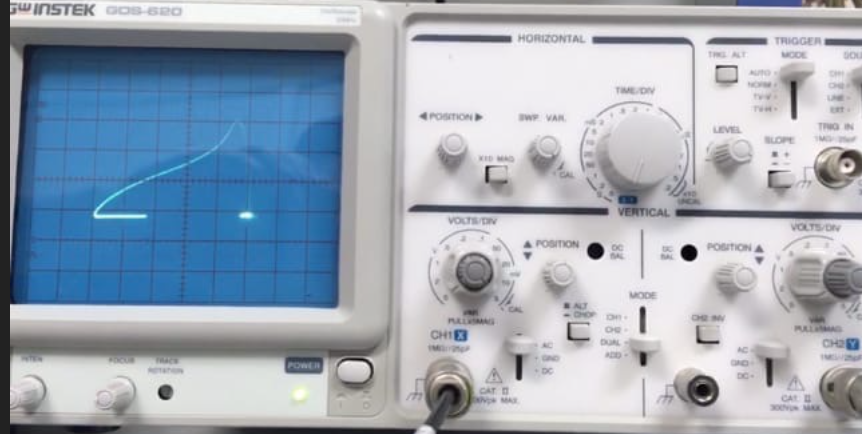
\includegraphics[width=0.7\textwidth]{a.jpg} 
\end{center}

Данной фазовой траектории можно однозначно сопоставить вольт-амперную характеристику стабилитрона. Сглаживание траектории обьясняется пренебрежениями, допущенными в ьеоретической модели, которыми нельзя было пренебрегать. Следует иметь в виду, что мы полностью прене- брегли паразитными емкостями и индуктивностями схемы. Не рассматривались также процессы развития разряда и деионизация при гашении.

\section{Выводы и рассчет погрешностей}

\subsection{Вывод}


Мы познакомились с работой релаксационного генератора и определили все характеризующие его параметры.  Выяснилось, что теоретические рассчеты немногим отличаются от действительности, например Динамический потенциал гашения отличается на 7\%. 

\subsection{Погрешности}

$$\frac{\Delta V_{д}}{V_{д}} = \sqrt{\left(\frac{\Delta U}{U} \right)^2 + \left(\frac{\Delta V_1}{V_1} \right)^2 + \left(\frac{\Delta R}{R} \right)^2 + \left(\frac{\Delta C}{C} \right)^2 + \left(\frac{\Delta T}{T} \right)^2} \approx  \frac{\Delta T}{T}  \approx 3\%$$

\end{document}
